\documentclass[a4paper,
    11pt,
    headings=small,
    ngerman,
    listof=totoc,
    numbers=noenddot]{scrreprt}[2021/11/13]
\usepackage{ifxetex,ifluatex}
\ifcase \ifxetex 1\else\ifluatex 1\else 0\fi\fi\usepackage[utf8]{inputenc}\fi
\usepackage[T1]{fontenc}
\usepackage[ngerman]{babel}
\usepackage[utf8]{inputenc}
\usepackage{setspace}
\onehalfspacing
\usepackage{lmodern}
\usepackage{csquotes}

\usepackage[automark,headsepline=.4pt]{scrlayer-scrpage}
\clearmainofpairofpagestyles
\pagestyle{scrheadings}
\renewcommand*{\chaptermarkformat}{%
	\chaptername~\thechapter\autodot\enskip}
\ihead{\headmark}
\setkomafont{pageheadfoot}{}
\renewcommand*{\sectionmarkformat}{}
\cfoot{\pagemark}
\footskip1cm

\usepackage[left=2.5cm,right=2.5cm,top=3cm,bottom=2.5cm]{geometry}

\usepackage{xcolor, soul}
\definecolor{codebackground}{rgb}{0.95, 0.95, 0.92}
\definecolor{Black}{rgb}{0, 0, 0}

%%% Für Abkürzungen und Abkürzungsverzeichnis %%%
\usepackage[printonlyused,withpage]{acronym}

%%% Für Mathe %%%
\usepackage[fleqn]{amsmath}
\usepackage{commath}
\usepackage{amstext}
\allowdisplaybreaks
%%% Für schräge Bruchstriche %%%
\usepackage{nicefrac}

%%% Für Quotes %%%
\usepackage{url}
\usepackage[ngerman]{varioref}
\usepackage{mwe}
\usepackage{hyperref}% Weil es so in der Frage enthalten war.
 \hypersetup{%draft, 								% no hyperlinking at all (useful in b/w printouts)
    colorlinks=true, breaklinks=true,
    urlcolor=Black, linkcolor=Black, citecolor=Black,
    linktoc=page, %
    bookmarksnumbered, bookmarksopenlevel=1, bookmarksdepth = section,%
    pdfstartview=FitV,
    }
\setlength{\parindent}{0em}
\usepackage{bookmark}% Weil das hyperref deutlich verbesser.
\usepackage{cleveref}
\crefname{paragraph}{Abschnitt}{Abschnitt}

%%% Für Textübergreifende Numerierung %%%
\usepackage{enumitem}
\renewcommand{\labelenumi}{\alph{enumi})}

%%% Um PDFs einzubinden %%%
\usepackage{pdfpages}

%%% Um Zahlen mit Einheiten korrekt darstellen %%%
\usepackage{siunitx}
\sisetup{
  locale = DE ,
  detect-all,
  binary-units = true
}

%%% Code schoen darstellen %%%
\usepackage{listings}
\lstdefinestyle{MyPythonStyle}{
  frame=tb, % hrule above and below
  keepspaces=true,
  breaklines=true,
  columns=flexible,
  basicstyle=\texttt\scriptsize,
  escapeinside={(*@}{@*)}, % for escaping
  backgroundcolor=\color{codebackground},
  showstringspaces=false,
  language=Python,
  keywordstyle=\color{blue},
  stringstyle=\color{red},
  commentstyle=\color{teal},
  numbers=left, % {none, left, right}
  firstnumber=1,
  numberstyle=\scriptsize\color{black},
  numbersep=5pt,
  xleftmargin=5.0ex,
  gobble=-4
}

%%% Korrekte darstellung fuer Sonderzeichen im Code
\lstset{literate=%
    {Ö}{{\"O}}1
    {Ä}{{\"A}}1
    {Ü}{{\"U}}1
    {ß}{{\ss}}1
    {ü}{{\"u}}1
    {ä}{{\"a}}1
    {ö}{{\"o}}1
    {~}{{\textasciitilde}}1
}


%%% Verzeichnisse im Anhang %%%
\DeclareNewTOC[%
  owner=\jobname,
  listname={Inhalt des Anhangs},% Titel des Verzeichnisses
]{atoc}% Dateierweiterung (a=appendix, toc=table of contents)
\DeclareNewTOC[%
  listname={Abbildungen im Anhang},% Titel des Verzeichnisses
]{alof}% Dateierweiterung (a=appendix, lof=list of figures)
\DeclareNewTOC[%
  listname={Tabellen im Anhang},% Titel des Verzeichnisses
]{alot}% Dateierweiterung (a=appendix, lot=list of tables)
 
\makeatletter
\newcommand*{\useappendixtocs}{%
  \renewcommand*{\ext@toc}{atoc}%
  \scr@ifundefinedorrelax{hypersetup}{}{% damit es auch ohne hyperref funktioniert
    \hypersetup{bookmarkstype=atoc}%
  }%
  \renewcommand*{\ext@figure}{alof}%
  \renewcommand*{\ext@table}{alot}%
}
\newcommand*{\usestandardtocs}{%
  \renewcommand*{\ext@toc}{toc}%
  \scr@ifundefinedorrelax{hypersetup}{}{% damit es auch ohne hyperref funktioniert
    \hypersetup{bookmarkstype=toc}%
  }%
  \renewcommand*{\ext@figure}{lof}%
  \renewcommand*{\ext@table}{lot}%
}
\scr@ifundefinedorrelax{ext@toc}{%
  \newcommand*{\ext@toc}{toc}
  \renewcommand{\addtocentrydefault}[3]{%
    \expandafter\tocbasic@addxcontentsline\expandafter{\ext@toc}{#1}{#2}{#3}%
  }
}{}
\makeatother
 
\usepackage{xpatch}
\xapptocmd\appendix{%
  \addpart{\appendixname}
  \useappendixtocs
}{}{}

%%% Alles bzgl. des Literaturverzeichnisses
\usepackage[bibencoding=utf8,
			sortlocale=de,
			style=numeric,
			pagetracker=true,
			autocite=inline,
			backrefstyle=three+,
			date=short,
			sorting=nty,
			backend=biber]{biblatex}
\bibliography{Literaturverzeichnis}

%%% urldate in eckigen Klammern %%%
\DeclareFieldFormat{urldate}{\mkbibbrackets{#1}}
%%% URL: = Verfügbar unter: %%%
\DeclareFieldFormat{url}{{Verfügbar unter:}\space\url{#1}}
%%% Abstand zwischen den Literaturangaben %%%
\setlength{\bibitemsep}{1.3em}
%%% statt und ein & %%%
\renewcommand*{\finalnamedelim}{\space\&\space}
%%% Nachname, Vorname, immer %%%
\DeclareNameAlias{sortname}{last-first}

\begin{document}
\pagenumbering{gobble}
\pagestyle{empty}


\begin{center}
  \Large{Berufliches Schulzentrum für Elektrotechnik Dresden}\\
\end{center}

\begin{center}
  \Large{Fachbereich Informationstechnik}
\end{center}
\begin{verbatim}

\end{verbatim}
\begin{center}
  \textbf{\LARGE{Projektdokumentation}}
\end{center}

\begin{center}
  \Large{Lernfeld 9 - Projekt 3}
\end{center}

\vspace{\fill}

\begin{flushleft}
  \begin{tabular}{lll}
                            &                                                & \\
                            &                                                & \\
                            &                                                & \\
                            &                                                & \\
                            &                                                & \\
                            &                                                & \\
    \textbf{Auftraggeber:}  & Doubtful-Joy SE                                & \\
    \textbf{Auftragnehmer:} & High-Secure GmbH - Projektteam IT20/2 Gruppe 7 & \\
    \textbf{Auftragsdatum:} & 2021.11.15                                     & \\
                            &                                                & \\
    \textbf{Historie:}
                            &                                                  \\
                            &                                                & \\
  \end{tabular}
\end{flushleft}

%%% Inhaltsverzeichnis
\tableofcontents

\newpage

%%% Abkürzungsverzeichnis %%%
\chapter*{Abkürzungsverzeichnis}
\addcontentsline{toc}{chapter}{Abkürzungsverzeichnis}

\begin{acronym}[DHCP]
  \acro{API}{Application Programming Interface}
  \acro{DB}{Datenbank}
  \acro{DHCP}{Dynamic Host Configuration Protocol}
  \acro{DNS}{Domain Name System}
  \acro{DMZ}{Demilitarisierte Zone}
  \acro{VM}{virtuelle Machine}
  \acrodefplural{VM}{virtuelle Machinen}
\end{acronym}

\newpage
\pagestyle{scrheadings}
\pagenumbering{arabic}
\ohead{Projekt 3, Lehrjahr 21/22}
\ihead{\rightmark}

%%% Was muss in ein Pflichtenheft: https://www.vario-software.de/lexikon/pflichtenheft/

\chapter{Pflichtenheft}

\section{Auftraggeber und Auftragnehmer }

Beim Auftraggeber handelt es sich um die Gaming-Plattform \textbf{Doubtful-Joy SE}. Ansprechpartner sind

\begin{table}[htbp]
  \centering
  \renewcommand{\arraystretch}{1.25}
  \caption{Ansprechpartner Auftraggeber}
  \begin{tabular}{lllll}
    Funktion     & Name   & Vorname & Email                                 \\
    \hline
    Auftraggeber & Hempel & Steffen & \flq{}hempel@bszetdd.lernsax.de\frq{} \\
  \end{tabular}
  \label{tab:Auftraggeber}
\end{table}

Beim Auftragnehmer handelt es sich um das \textbf{High-Secure GmbH - Projektteam IT20/2 Gruppe 7}. Ansprechpartner sind

\begin{table}[htbp]
  \centering
  \renewcommand{\arraystretch}{1.25}
  \caption{Ansprechpartner Auftragnehmer}
  \begin{tabular}{lllll}
    Funktion          & Name      & Vorname  & Email                                         \\ \hline
    Projektmanager    & Egermann  & Péter    & \flq{}i20egermannpe@bszetdd.lernsax.de\frq{}  \\
    Teamleiter        & Leyrer    & Johannes & \flq{}i20leyrerjo@bszetdd.lernsax.de\frq{}    \\
    Netzwerkingenieur & Brethfeld & Vinzenz  & \flq{}i20brethfeldvi@bszetdd.lernsax.de\frq{} \\
  \end{tabular}
  \label{tab:Auftragnehmer}
\end{table}


\section{Ausgangslage}

Die existierende Support-Infrastruktur der Gaming-Plattform Doubtful-Joy SE lässt sich über Mail und Telefon kontaktieren. Dabei wird jeder Anruf und jede Mail individuell von einem Mitarbeiter als Ticket gespeichert und in einem zentralen Laufwerk abgelegt. Effizienz, Ordnung und Übersichtlichkeit sind nicht ausreichend vorhanden.


\section{Projektziel}

Die Gaming-Plattform Doubtful-Joy SE möchte ihre existierende Support-Infrastruktur durch ein Ticketsystem ersetzen. Dieses soll für Kunden und Mitarbeiter über ein Web-Interface erreichbar sein. Tickets sollen über dieses direkt erstellt und mit beliebig vielen Attachments versehen werden können.

Außerdem soll eine Segmentierung der Netzinfrastruktur mit einer sichereren Trennung von öffentlich erreichbaren Diensten und dem Intranet eingerichtet werden. Ebenso sollen die internen Dienste \ac{DNS} und \ac{DHCP} auf einem separatem System bereitgestellt werden, um eine Abhängigkeit von der Firewall auszuschließen.

Doubtful-Joy SE setzt auf RedHat und binärkompatible Systeme, weshalb diese System-Strategie weiterhin umgesetzt werden soll.


\section{Funktionsspezifikation}

Von der Realisierung sind betroffen:

\begin{description}
  \item[Manware] \
    \begin{itemize}
      \item Projektteam IT20/2 Gruppe 7
      \item Support-Mitarbeiter des Auftraggeber
      \item IT-Mitarbeiter des Autraggebers
    \end{itemize}
  \item[Orgware] \
    \begin{itemize}
      \item Sicherheitsanforderungen
      \item Benutzerhandbuch
      \item Benutzerschulung
    \end{itemize}
  \item[Hardware] \
    \begin{itemize}
      \item Server
      \item Mitarbeiter-PCs
    \end{itemize}
  \item[Software] \
    \begin{itemize}
      \item VM-Ware
      \item Datenbank-Server
      \item Web-Server
      \item Firewall-System
      \item \ac{DNS}
      \item \ac{DHCP}
    \end{itemize}
\end{description}


\section{Datenspezifikation}

Da von etwa 1000 Telefonanrufen  und Emails pro Tag ausgegangen wird, kann dies etwa 1:1 in 1000 Tickets übertragen werden. Der Speicherbedarf pro Ticket wird hier im Schnitt auf etwa \SI{5}{\mega\byte} geschätzt, da wahrscheinlich häufiger Anhänge in Bildform zur besseren Problembeschreibung genutzt werden. Zusätzlich wird davon ausgegangen, dass die Daten zur Sicherheit und Nachvollziehbarkeit für ein Jahr gespeichert werden, wodurch die Datenbank \SI{1830}{\giga\byte} Speicher in einem Jahr benötigt.

\begin{align*}
  \frac{\SI{5}{\mega\byte}}{\text{Ticket}} \cdot \frac{1000\text{ Ticket}}{\text{Tag}} & = \frac{\SI{5000}{\mega\byte}}{\text{Tag}}                                                                  \\
  \frac{\SI{5000}{\mega\byte}}{\text{Tag}} \cdot 365 \text{Tage}                       & = \frac{\SI{1825000}{\mega\byte}}{\text{Jahr}} \stackrel{\wedge}= \frac{\SI{1830}{\giga\byte}}{\text{Jahr}}
\end{align*}


Da es keine Good-Practice ist, die Bilder in der Datenbank zu speichern, wird nur der Dateipfad zu den Bildern in der Datenbank hinterlegt, die Bilder selbst liegen auf der Festplatte des Webservers. Damit verringert sich der geschätzte Speicherbedarf der Datenbank auf etwa \SI{183}{\giga\byte} pro Jahr.

\begin{align*}
  \frac{\SI{0.5}{\mega\byte}}{\text{Ticket}} \cdot \frac{\text{Ticket}}{\text{Tag}} = \frac{\SI{500}{\mega\byte}}{\text{Tag}} \stackrel{\wedge}= \frac{\SI{183}{\giga\byte}}{\text{Jahr}}
\end{align*}

Die Bilder selbst benötigen zum aktuellen Stand auf der Festplatte \SI{1643}{\giga\byte} Speicher pro Jahr.

\begin{align*}
  \frac{\SI{4.5}{\mega\byte}}{\text{Bild}} \cdot 1000 \frac{\text{Bild}}{\text{Tag}} = \frac{\SI{4500}{\mega\byte}}{\text{Tag}} \stackrel{\wedge}= \frac{\SI{1643}{\giga\byte}}{\text{Jahr}}
\end{align*}

Die Art von Daten sind personenbezogene Daten in Text- und Bildform.

Der Datenfluss geht vom Clienten zur \ac{DMZ} und zur Bearbeitung dann zum PC des Support-Mitarbeiters, grafisch dargestellt in \vref{fig:Schnittstellenspezifikation}.


\newpage
\section{Schnittstellenspezifikation}

\begin{figure}[htbp]
  \centering
  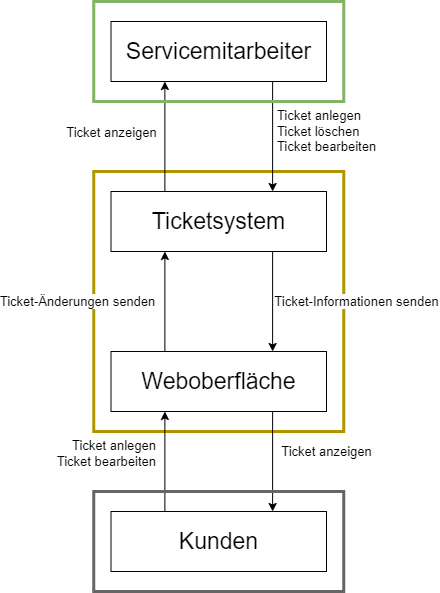
\includegraphics[width=0.75\textwidth]{data/Schnittstellendiagramm.png}
  \caption{Schnittstellenspezifikation}
  \label{fig:Schnittstellenspezifikation}
\end{figure}


\section{Rahmenbedigungen}

Der Auftraggeber hat folgende Ressourcen bereitzustellen und Mitwirklungspflichten:

\begin{itemize}
  \item Server
  \item Mitarbeiter-PCs
  \item Zugriff auf alle zu bearbeitenden Systeme und Zutritt zu den notwendigen Räumlichkeiten
  \item Kooperation und eventuell notwendigen lokalen Support
\end{itemize}


\section{Qualitätsbetrachtung}

Die Arbeitspakete werden stets während der Bearbeitung sowie nach der Fertigstellung auf Funktion und Qualität überprüft.

Wöchentlich werden Meetings abgehalten um den Stand des Projekts zu erörtern und auf eventuell auftretende Probleme zeitnah reagieren zu können.

Die Zeitplanung und damit der Aufwand ist in \vref{fig:Gantt} in kleinem Format und groß in \vref{fig:Gantt} zu sehen.  Für einen langfristigen Support für nach der der Fertigstellung wird ein zusätzliches Angebot vorgelegt.


\section{Projektplanung}

Die Projektplanung ist im Projektstrukturplan, zu sehen in \vref{fig:Projektstrukturplan}, und im Gantt-Diagramm, zu sehen in \vref{fig:GanttKlein}, bzw. \vref{fig:Gantt}, abgebildet.
Ebenso wird der im Anhang \cpageref{fig:Netzwerkplan} zu betrachtende Netzwerkplan \vref{fig:Netzwerkplan} umgesetzt.

\begin{figure}[htbp]
  \centering
  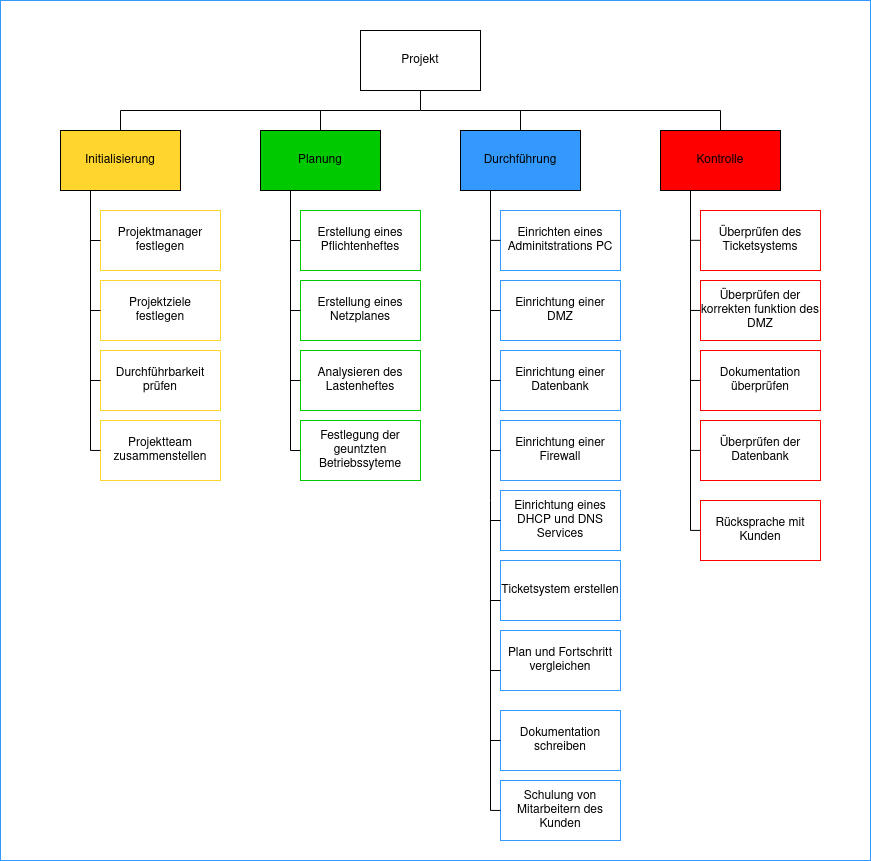
\includegraphics[width=0.75\textwidth]{data/Projektstrukturplan.png}
  \caption{Projektstrukturplan}
  \label{fig:Projektstrukturplan}
\end{figure}

\begin{figure}[htbp]
  \centering
  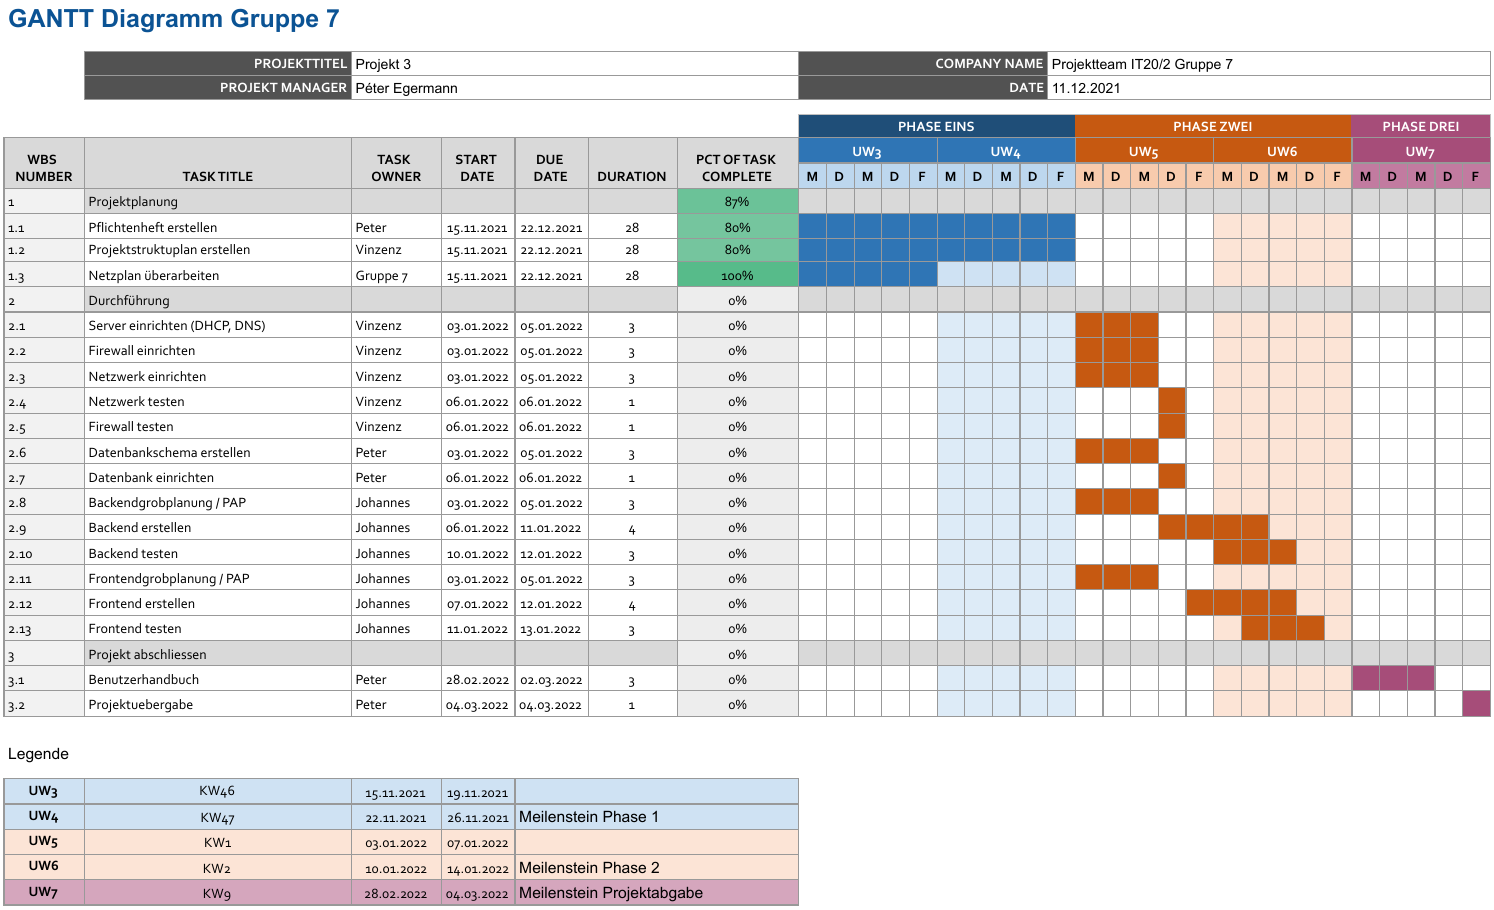
\includegraphics[width=0.95\textwidth]{data/Gantt.png}
  \caption{Gantt-Diagramm}
  \label{fig:GanttKlein}
\end{figure}


\section{Kosten-Nutzen-Analyse}

Eine Kosten-Nutzen-Analyse ist zum jetzigen Zeitpunkt nicht notwendig, da der Support erst mal entlastet werden muss. Dies ist durch das neue System auf jeden Fall der Fall, da quasi der Kunde das Ticket erstellt und nicht der Support-Mitarbeiter. Somit kann sich voll auf das Beheben des Problems konzentriert werden.


\chapter{Auswertung und Reflexion}

\section{Ablaufdokumentation}

In diesem Projekt wurden drei Netze eingerichtet, um ein echtes Netzwerk wiederzugeben. Dabei handelt es sich um das rote Netz, das das Internet wiedergeben soll, das orange Netz, was eine sogenannte \ac{DMZ} darstellt und das grüne Netz, das das interne Netz darstellt.
Um die Kommunikation und den Zugriff zwischen den Netzen zu regeln wird in diesem Projekt die Firewall verwendet. Somit kann aus dem roten Netz nur mit dem orangen Netz kommunizieren werden, aus dem grünen Netz ist kein Zugriff auf das Internet möglich und zwischen dem orangen und grünen Netz sind nur bestimmte Ports zur Kommunikation und Datenübertragung zugelassen.

Um Maschinen in den verschiedenen Netzen darzustellen wurden vier verschiedene \acp{VM} aufgesetzt, die bis auf der IPFire auf CentOS 8 Stream basieren:

\begin{itemize}
  \item IPFire (als Knotenpunkt für alle drei Netze)
  \item Admin-PC (grünes Netz)
  \item \ac{DHCP}-\ac{DNS}-\ac{DB}-Server (grünes Netz)
  \item Webserver (\ac{DMZ}, oranges Netz)
\end{itemize}


\section{Einrichtung IPFire}

Vor dem Einrichten der IPFire müssen noch zwei Netzwerke zu dem schon bestehenden Netzwerk hinzugefügt werden, da die Firewall mit drei verschiedenen Netzen interagieren soll. Noch dazu werden den einzelnen Netzen verschiedene MAC-Adressen zugeteilt, damit sie in der späteren Nutzung zuordenbar sind.

In unserem Projekt wurden die Netzwerke wie in \vref{tab:Netzwerk} zu sehen verteilt.

\begin{table}[htbp]
  \centering
  \renewcommand{\arraystretch}{1.25}
  \caption{Netzwerkauslegung}
  \begin{tabular}{lll}
    Netzwerk-Farbe & MAC-Adresse       & Netzwerk \\
    \hline
    Rot            & 00:50:56:32:BA:0F & NAT      \\
    Grün           & 00:50:56:3D:EC:D6 & VMnet1   \\
    Orange         & 00:50:56:3E:56:B7 & VMnet2   \\
  \end{tabular}
  \label{tab:Netzwerk}
\end{table}

Als Hostname der Firewall wurde "ipfire" und als Domaine wurde "doubtful-joy07.com" festgelegt.
Nach dem Auswählen der Sprache wurde aufgrund der Kundenspezifikation das Filesystem "ext4 Filesystem" ausgewählt. Nach dem Zuweisen der einzelnen Netze mit den IP- und MAC-Adressen wurde der \ac{DHCP} deaktiviert, damit es später mit dem \ac{DHCP}-Server im grünen Netz nicht zu Komplikationen führt.

Nachdem die Firewall eingerichtet wurde können aus dem grünen Netz mittels des IPFire-WebInterfaces verschiedene Einstellungen der Firewall
bearbeitet werden. Für die Verbindungen zwischen Admin-PC, \ac{DHCP}-\ac{DNS}-\ac{DB}-Server und Webserver sowie für die Erreichbarkeit des Webservers aus dem roten Netz wurden vier verschiedene Regeln erstellt, die in n \vref{fig:FirewallConfig} zu sehen sind.

\begin{figure}[htbp]
  \centering
  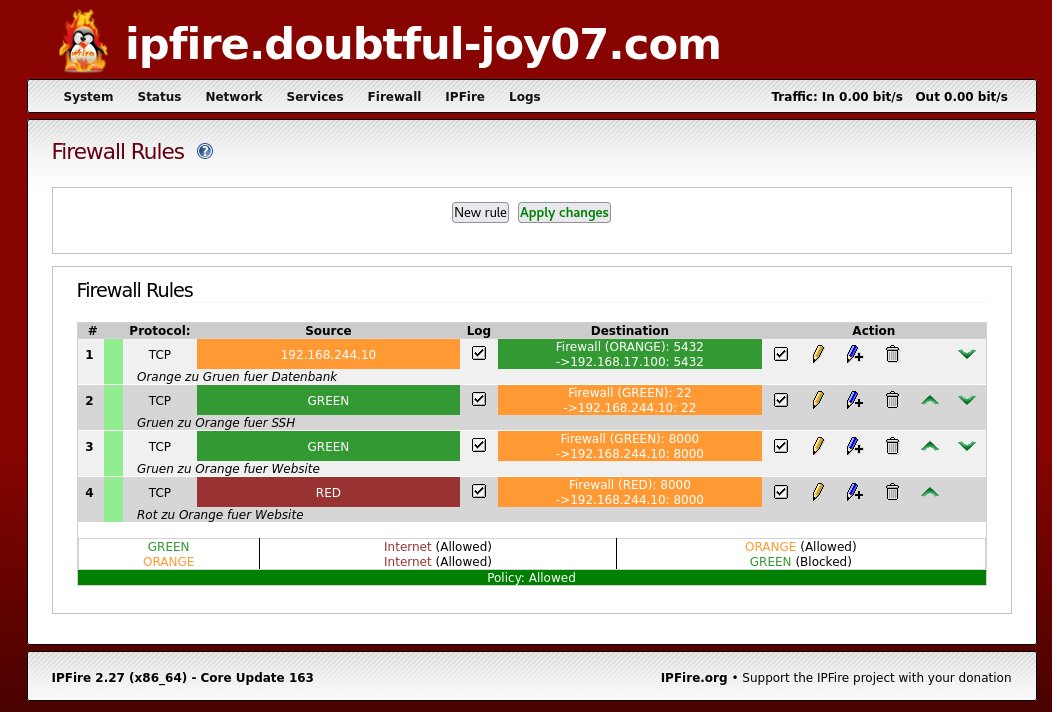
\includegraphics[width=0.95\textwidth]{data/ipfire-config.png}
  \caption{Firewall-Regeln}
  \label{fig:FirewallConfig}
\end{figure}

Die erste Regel dient der Kommunikation zwischen Webserver (\ac{DMZ}) und Datenbank (grünes Netz), sodass Tickets abgerufen und gespeichert werden können. Damit aus dem grünen Netz der Webserver gestartet und gestoppt werden kann, wurde Regel 2 implementiert. Die Erreichbarkeit des WebInterface der Ticket-Seite durch die Mitarbeiter aus dem grünen Netz wurde mit Regel 3 erreicht. Die letzte Regel erlaubt den Zugriff aus dem Internet auf die Ticket-Website.


\section{Einrichtung Admin-PC}

Nach der Standard-Installation von CentOS 8 Stream wurden das Netzwerk der \ac{VM} angepasst. Hier wurde der \ac{DNS} auf die IP-Adresse des \ac{DHCP}-\ac{DNS}-\ac{DB}-Servers gesetzt.

Da in CentOS 8 Stream SSH-Client und -Server bereits installiert und aktiviert sind, konnte der Webserver direkt angesprochen werden. Dies erfolgte ueber das Gateway des grünen Netzes, wie in \vref{fig:PythonScriptRunning} zu sehen. Um zu sehen, ob der Webserver aktiv ist, können mittels \texttt{ps -ef | grep python} alle laufenden Python-Anwendungen aufgelistet werden, was ebenfalls in \vref{fig:PythonScriptRunning} zu sehen ist.

\begin{figure}[htbp]
  \centering
  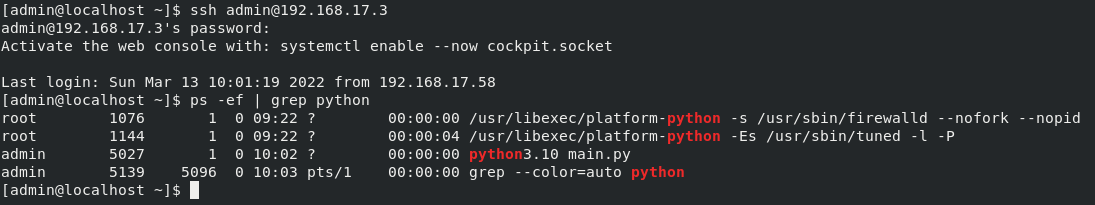
\includegraphics[width=0.95\textwidth]{data/py-script-running.png}
  \caption{SSH-Login sowie Auflisten aller laufenden Python-Anwendungen}
  \label{fig:PythonScriptRunning}
\end{figure}

Ist der Webserver aktiv und soll gestoppt werden, kann mittels \texttt{ps -ef | grep python} die ID des Scripts ermittelt und mittels \texttt{kill -9 ID} gestoppt werden. Dies ist in \vref{fig:PythonScriptStop} zu sehen.

\begin{figure}[htbp]
  \centering
  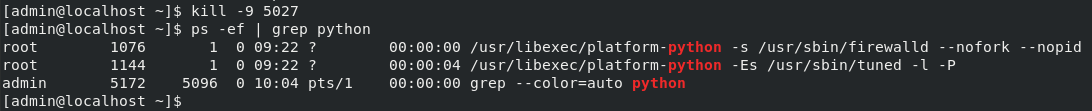
\includegraphics[width=0.95\textwidth]{data/py-script-admin-stop.png}
  \caption{Stoppen einer bestimmten Python-Anwendungen}
  \label{fig:PythonScriptStop}
\end{figure}

Soll der Webserver gestartet werden, kann dies mittels Navigation in den Ordner, in dem die auszuführende Datei liegt und \texttt{python3.10 name-der-datei \&} gestartet werden, zu sehen in der \vref{fig:PythonScriptStart}. Das \& erlaubt das Laufen der Anwendung im Hintergrund und wird so nicht gestoppt, wenn die SSH-Verbindung geschlossen wird.

\begin{figure}[htbp]
  \centering
  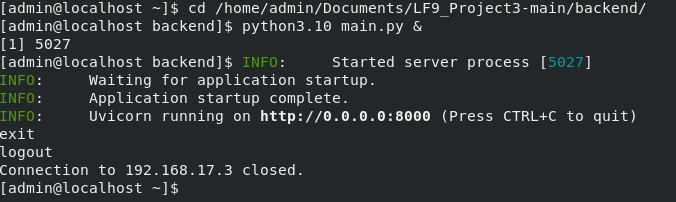
\includegraphics[width=0.95\textwidth]{data/py-script-admin-start.png}
  \caption{Starten einer bestimmten Python-Anwendungen}
  \label{fig:PythonScriptStart}
\end{figure}


\section{Einrichtung DHCP-DNS-DB-Server}


\section{Einrichtung Webserver}


\newpage

%%% Abbildungsverzeichnis
\listoffigures
%%% Tabellenverzeichnis
\listoftables
%%% Codeverzeichnis
\lstlistoflistings

\newpage

\appendix
\ihead{Anhang}


\chapter{Gantt-Diagramm}

\begin{figure}[h!]
  \centering
  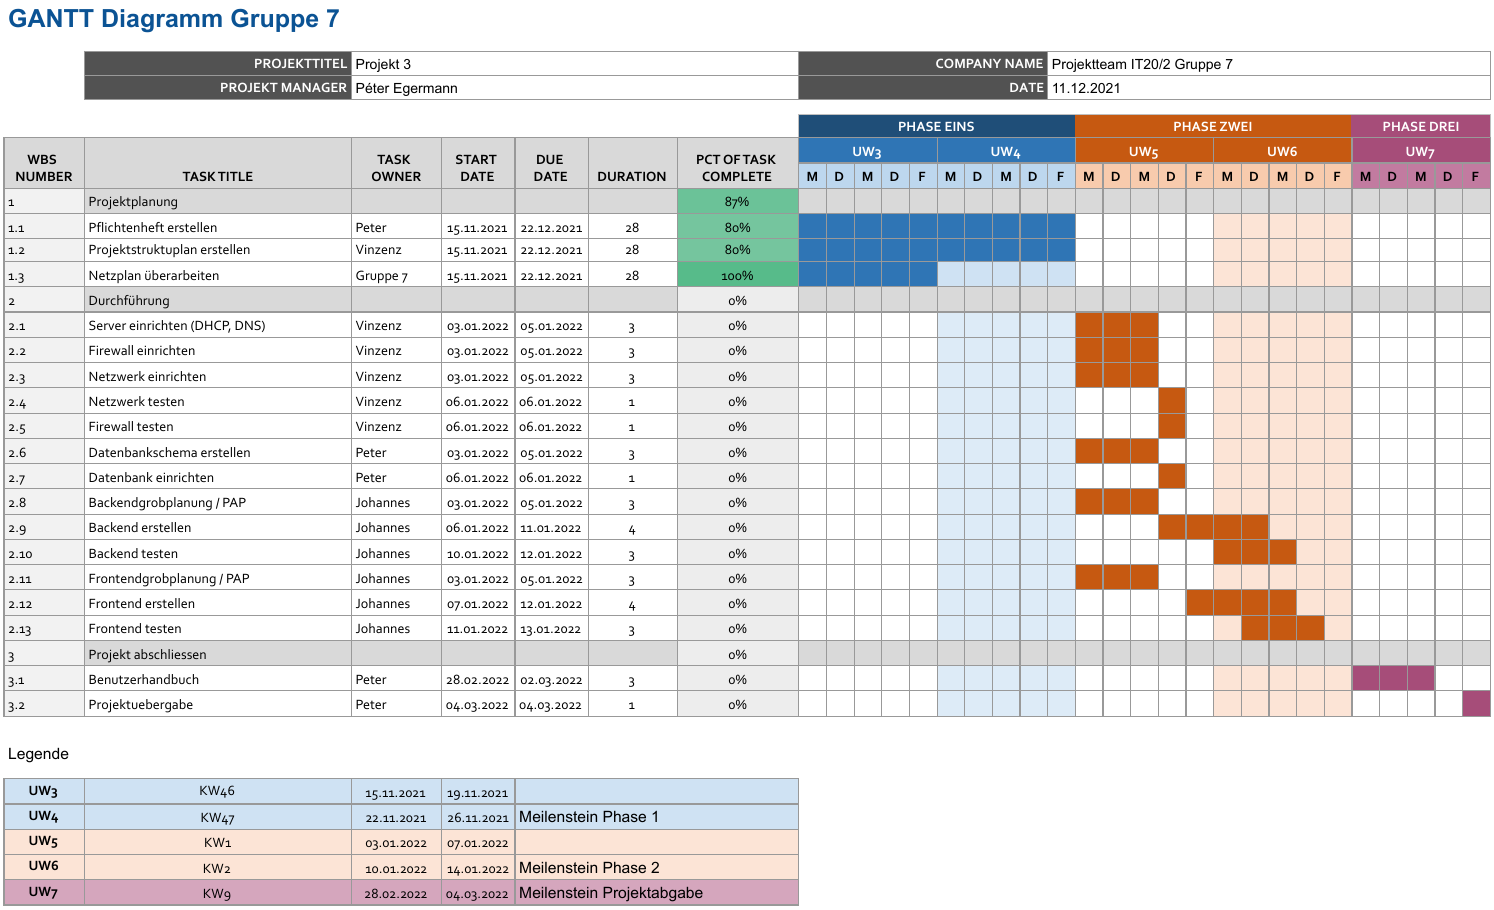
\includegraphics[angle=90,origin=c,width=0.75\textwidth]{data/Gantt.png}
  \caption{Gantt-Diagramm}
  \label{fig:Gantt}
\end{figure}


\chapter{Netzwerkplan}

\begin{figure}[h!]
  \centering
  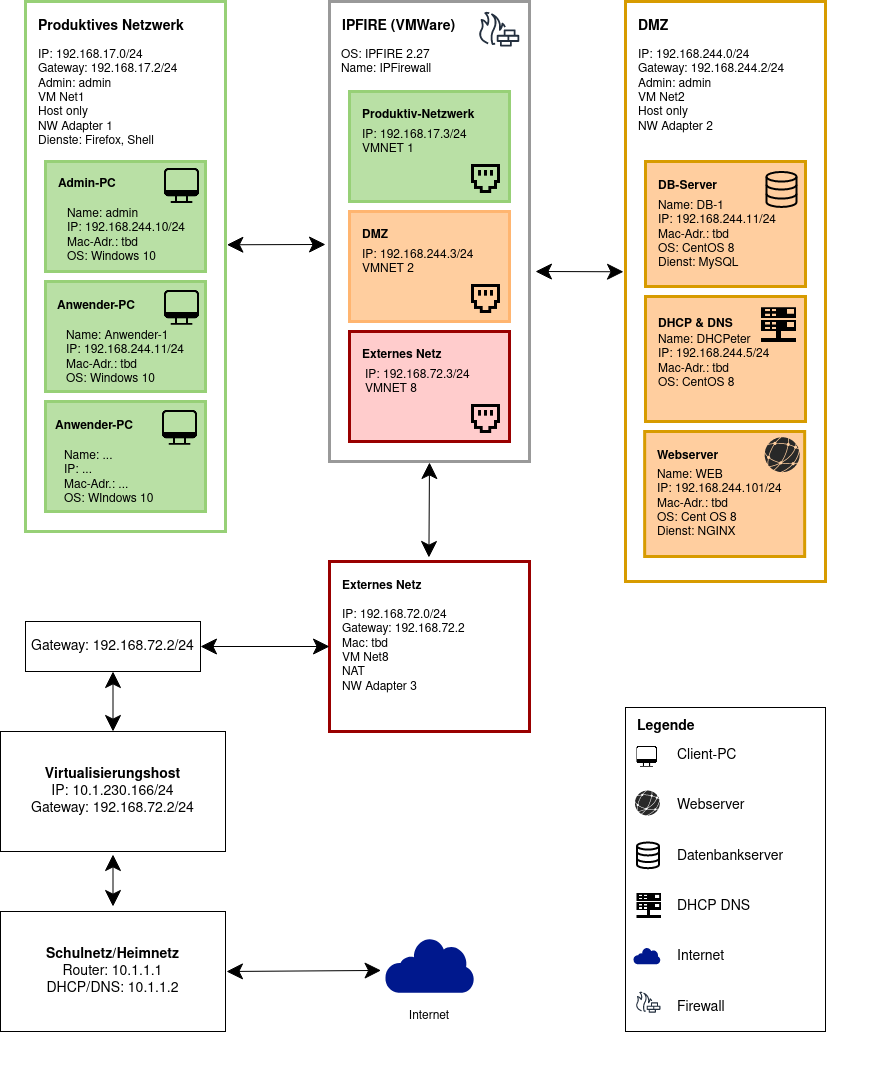
\includegraphics[width=0.95\textwidth]{data/Netzwerkplan.png}
  \caption{Netzwerkplan}
  \label{fig:Netzwerkplan}
\end{figure}

\end{document}
